% Исходный LaTeX-код (c) Пётр Калинин
% Код распространяется по лицензии GNU GPL (!)

\header{Элементарная реализация и общие замечания}
\lheader{Реализация} Итак, что такое поиск в глубину. Поиск в глубину "--- это рекурсивный алгоритм обхода графа.
Он принимает на вход некоторую вершину графа и рекурсивно запускает себя для всех ещё не посещённых 
соседей данной вершины. Таким образом, у нас в каждый момент про каждую вершину мы знаем, были мы в 
ней уже или ещё нет. При входу в очередную вершину мы помечаем, что мы в ней были, и рекурсивно 
входим во все соседние с ней вершины, в которых ещё не были. Элементарная реализация поиска в 
глубину тогда получает следующий вид (считаем, что мы храним граф матрицей смежности):

\begin{codesampleo}\begin{verbatim}
procedure find(i:integer);
begin
was[i]:=1;
for j:=1 to n do
    if (gr[i,j]=1)and(was[j]=0) then
       find(j);
end;
\end{verbatim}
\end{codesampleo}
Здесь $gr$ "--- матрица смежности, $was$ "--- тот самый массив, в котором мы храним, были мы уже в 
этой вершине или нет ещё.

В принципе, это абсолютно корректный вариант реализации, но я лично предпочитаю другой вариант: как 
в любых рекурсивных процедурах, я предпочитаю проверять необходимость рекурсивного вызова при 
\textit{входе} в процедуру, а не \textit{при её вызове} (конечно, пока это возможно). Конкретно, в 
данном случае я предпочитаю перекинуть проверку $was[j]=0$ в начало процедуры:
\begin{codesampleo}\begin{verbatim}
procedure find(i:integer);
begin
if was[i]<>0 then
   exit;
was[i]:=1;
for j:=1 to n do
    if gr[i,j]=1 then
       find(j);
end;
\end{verbatim}
\end{codesampleo}
(обратите внимание, что, конечно, проверка из $was[j]$ превратилась в $was[i]$).

Смысл такого переноса проверок в общем случае рекурсивных процедур (в первую очередь в случае 
перебора) в том, что 1. если вы вызываете вашу процедуру из нескольких мест в коде, то не надо 
каждый раз дублировать проверку, 2. нередко в начале процедуры проверка смотрится как-то 
естественнее (естественнее по максимуму работать с $i$-ой вершиной, т.к. именно она является 
параметром процедуры), и иногда эту проверку тут написать проще. С другой стороны, такой перенос 
приводит к дополнительным затратам времени на вызов функции при выполнении программы, но по"=моему 
в большинстве случаев эти затраты несущественны (время выполнения самой процедуры обычно много 
больше). Правда, в случае поиска в глубину все эти преимущества почти незаметны, т.к. $was[i]<>0$ 
"--- фактически единственная проверка, которую получается перенести (совершенно понятно, что 
проверку $gr[i,j]=1$ переносить невозможно и вообще бессмысленно), к тому же процедура find обычно 
вызывается максимум из двух мест в коде, поэтому экономии от переноса нет, так что здесь это скорее 
дело вкуса.

Ещё обращу внимание на то, что во втором варианте написано $was[i]<>0$, а не $was[i]=1$. Вообще, 
это как бы ещё пример общей идеи, что имхо стоит максимально расширять условия в if'ах. В данном 
случае потом может оказаться, что, зайдя в вершину, в was мы сохраним что"=нибудь ещё, не 
обязательно единицу (например, номер компоненты связности, или "<состояние"> вершины в том или ином 
смысле) "--- но в любом случае ноль будет обозначать непосещённую вершину, а не"=ноль "--- 
посещённую, поэтому $was[i]<>0$ будет всегда работать.

\lheader{Как вызывать процедуру $find$} 
\label{howtocall}
Конечно, сама по себе процедура ничего не сделает; чтобы её 
использовать, нужно её вызвать в главной программе (или, естественно, в другой процедуре, где вам 
понадобилось запустить поиск в глубину, и т.п.). Способ вызова, конечно, зависит от задачи, но 
наиболее часто используются два варианта: либо нужно просто запустить поиск в глубину из данной 
вершины и всё "--- это, естественно, делается просто вызовом $find(i)$, где $i$ "--- номер этой 
вершины, либо нужно запустить поиск так, чтобы обойти обязательно все вершины "--- тогда пишем так:
\begin{codesampleo}\begin{verbatim}
for i:=1 to n do
    if was[i]=0 then
       find(i);
\end{verbatim}
\end{codesampleo}
Конечно, если сам поиск написан вторым способом (т.е. с проверкой $was$ при входе в процедуру), то 
if из этого кода можно убрать.

И ещё, конечно, нужно не забыть предварительно занулить массив $was$.


\vspace{3cm}

\textit{(Продолжение на следующей странице)}

\eject
\lheader{Пример работы}
Пусть у нас есть граф, показанный на рис. Запустим на нем поиск в глубину из вершины 1. Пусть (в 
соответствии с тем, как это написано в приведённых выше реализациях) при  
просмотре соседних вершим мы перебираем вершины в порядке возрастания номеров. Тогда алгоритм 
поиска будет работать следующим образом (отступ строки соответствует уровню рекурсии):

\begin{wrapfigure}{r}{3cm}
\vspace{-0.3cm}
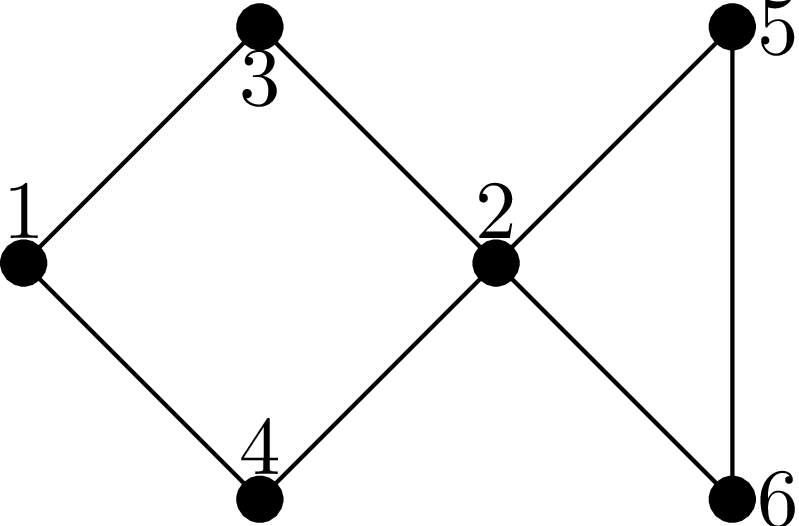
\includegraphics[width=3cm]{texts/04_1_dfs/graph.1}
\end{wrapfigure}
{\newcommand{\ind}{\hspace*{1cm}}\footnotesize

\noindent \texttt{find(1)}: запускаем поиск в глубину из вершины 1\\
Помечаем, что побывали в вершине 1\\
Просматриваем соседей вершины 1\\
Нашли соседа: вершину 2\\
В вершине 2 ещё не были\\
\ind \texttt{find(2)}: запускаем поиск в глубину из вершины 2\\
\ind Помечаем, что побывали в вершине 2\\
\ind Просматриваем соседей вершины 2\\
\ind Нашли соседа: вершину 1\\
\ind В вершине 1 уже были, поиск из вершины 1 не запускаем%
       \footnote{Или, если реализовано вторым 
         способом, запускаем, но тут же выходим назад.}%
        \\
\ind Нашли соседа: вершину 3\\
\ind В вершине 3 ещё не были\\
\ind \ind \texttt{find(3)}: запускаем поиск в глубину из вершины 3\\
\ind \ind Помечаем, что побывали в вершине 3\\
\ind \ind Просматриваем соседей вершины 3\\
\ind \ind Нашли соседа: вершину 1\\
\ind \ind В вершине 1 уже были, поиск из вершины 1 не запускаем\\
\ind \ind Нашли соседа: вершину 2\\
\ind \ind В вершине 2 уже были, поиск из вершины 2 не запускаем\\
\ind \ind Соседи вершины 3 закончились, завершаем поиск из вершины 3\\
\ind \textit{(продолжаем просмотр соседей вершины 2)}%
       \footnote{Обратите внимание, что это происходит автоматически: работа процедуры 
              \texttt{find(3)} завершилась, поэтому продолжается работа программы с того места, 
              откуда была вызвана процедура \texttt{find(3)} "--- а это есть строчка в цикле в 
              процедуре \texttt{find(2)}, поэтому просто происходит переход к следующей итерации 
              цикла в \texttt{find(2)}, т.е. продолжаем просмотр соседей вершины~2. Поэтому эта строчка здесь и написана 
              курсивом "--- ей, можно сказать, не соответствует никакая строка исходного текста 
              программы.}%
              \\
\ind Нашли соседа: вершину 4\\
\ind В вершине 4 ещё не были\\
\ind \ind \texttt{find(4)}: запускаем поиск в глубину из вершины 4\\
\ind \ind Помечаем, что побывали в вершине 4\\
\ind \ind Просматриваем соседей вершины 4\\
\ind \ind Нашли соседа: вершину 1\\
\ind \ind В вершине 1 уже были, поиск из вершины 1 не запускаем\\
\ind \ind Нашли соседа: вершину 2\\
\ind \ind В вершине 2 уже были, поиск из вершины 2 не запускаем\\
\ind \ind Соседи вершины 4 закончились, завершаем поиск из вершины 4\\
\ind \textit{(продолжаем просмотр соседей вершины 2)}\\
\ind Соседи вершины 2 закончились, завершаем поиск из вершины 2\\
\textit{(продолжаем просмотр соседей вершины 1)}\\
\dots{} (нашли соседей: вершины 3 и 4, поиск из них не запускаем, для краткости не описываю это подробно)\\
Нашли соседа: вершину 5\\
В вершине 5 ещё не были\\
\ind \texttt{find(5)}: запускаем поиск в глубину из вершины 5\\
\ind Помечаем, что побывали в вершине 5\\
\ind Просматриваем соседей вершины 5\\
\ind Нашли соседа: вершину 1\\
\ind В вершине 1 уже были, поиск из вершины 1 не запускаем\\
\ind Нашли соседа: вершину 6\\
\ind В вершине 6 ещё не были\\
\ind \ind \texttt{find(6)}: запускаем поиск в глубину из вершины 6\\
\ind \ind Помечаем, что побывали в вершине 6\\
\ind \ind Просматриваем соседей вершины 6\\
\ind \ind Нашли соседа: вершину 1\\
\ind \ind В вершине 1 уже были, поиск из вершины 1 не запускаем\\
\ind \ind Нашли соседа: вершину 5\\
\ind \ind В вершине 5 уже были, поиск из вершины 5 не запускаем\\
\ind \ind Соседи вершины 6 закончились, завершаем поиск из вершины 6\\
\ind \textit{(продолжаем просмотр соседей вершины 5)}\\
\ind Соседи вершины 5 закончились, завершаем поиск из вершины 5\\
\textit{(продолжаем просмотр соседей вершины 1)}\\
Нашли соседа: вершину 6\\\nopagebreak
В вершине 6 уже были, поиск из вершины 6 не запускаем\\\nopagebreak
Соседи вершины 1 закончились, завершаем поиск из вершины 1\\

}
\pagebreak[3]

На самом деле очень нетривиально придумать один небольшой пример, который бы полностью характеризовал все 
особенности поиска в глубину. Поэтому, если вам что-то во внутреннем механизме работы поиска ещё не 
понятно, порисуйте ещё графы и промоделируйте вручную работу поиска на них.

\lheader{Дерево поиска в глубину} У каждой вершины, кроме той, из которой был произведён начальный 
запуск поиска ("<корня">), можно выделить "<родителя"> "--- вершину, из которой мы перешли в данную вершину. 
Соединив каждую вершину (кроме корня, конечно) с её родителем, получим подграф исходного графа "--- 
\textit{дерево поиска в глубину}.

\task|Докажите, что действительно получится дерево. Точнее, докажите, что в полученном 
подграфе не будет циклов. Верно ли, что это всегда будет дерево, покрывающее все вершины исходного 
графа? Как это зависит от того, как мы вызываем поиск в глубину (п. \ref{howtocall})? На самом деле 
доказательство не очень тривиально.%
||||То, что не будет циклов, видимо, можно доказывать многими способами. Приведу идею
самого простого из пришедших мне сейчас в голову доказательств. Пронумеруем все вершины в том порядке, 
в котором мы их находили. В дереве поиска в глубину из каждой вершины $u$ выходим несколько (ноль или больше)
рёбер в её "<сыновья"> "--- вершины, которые мы нашли из $u$, значит, их номера больше, чем у $u$, "---
а также ровно одно ребро в "<предка"> "--- вершину, \textit{из} которой мы нашли $u$ (такие ребра есть
у всех вершин, кроме корня) "--- номер этой вершины меньше, чем у $u$. Пусть есть цикл. Рассмотрим в нем вершину с 
наибольшим номером. В неё входят \textit{два} ребра, принадлежащие этому циклу, и потому идущие и вершин с \textit{меньшими}
номерами, чем у нашей. Противоречие.

В случае связного графа это всегда будет остовное дерево графа, т.е. покрывающее все вершины. Но в случае
несвязного графа это будет или остовное дерево одной компоненты связности "--- если запускаем просто $find(i)$,
"--- или остовный лес, покрывающий все вершины "--- если запускаем вторым из перечисленных в п. \ref{howtocall}
способом.
|\label{provetree}

\begin{wrapfigure}[5]{r}{3cm}
\vspace{-0.7cm}
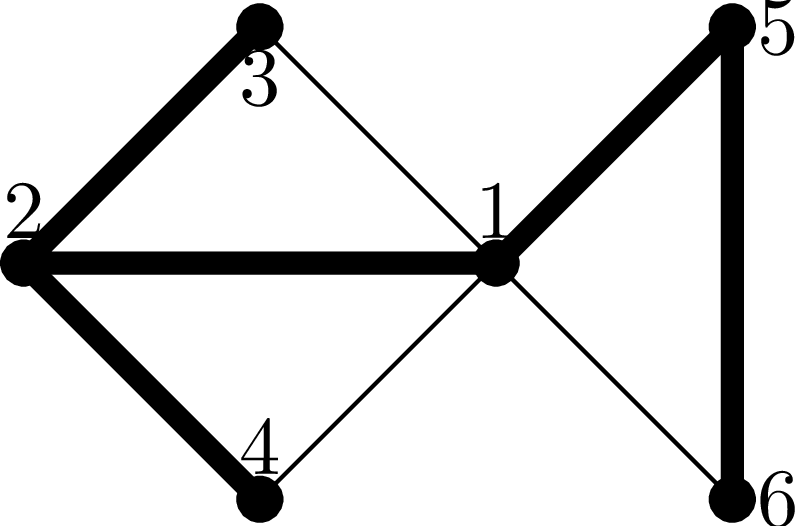
\includegraphics[width=3cm]{texts/04_1_dfs/graph.2}
\end{wrapfigure}

На рис. справа приведено дерево для примера из предыдущего пункта.

Собственно, поиск в глубину "--- самый, пожалуй, простой алгоритм построения в связном графе 
\textit{остовного} дерева (т.е. дерева, покрывающего все вершины графа). Если вам зачем"=то 
понадобилось \textit{любое} остовное дерево, пользуйтесь поиском в глубину. Кроме того, дерево 
поиска в глубину нам ещё пригодится при решении задач ниже.

\lheader{Оценка сложности}
Какова сложность поиска в глубину? Во"=первых, замечу, что здесь, как и на любых задачах на графы, 
1. сложность принято оценивать как функцию \textit{двух} параметров "--- количества вершин $V$ и 
количества рёбер $E$, и 2. сложность зависит от того, каким образом мы храним граф в памяти.

В первом варианте реализации очевидно, что процедура $find$ ни для какого параметра не будет 
вызвана дважды (т.е. $find(1)$ будет вызвана максимум один раз за время работы программы, $find(2)$ 
тоже максимум один раз и т.д.), поскольку перед каждым вызовом мы проверяем, а не были ли мы уже в этой 
вершине\footnote{Конечно, подразумевается, что вызов процедуры $find$ из главной программы сделан 
соответствующим образом "--- чтобы не получилось, что процедура будет дважды запущена с одним и тем 
же параметром}. Поэтому общее количество вызовов будет $O(V)$. Сложность работы каждой процедуры 
(не считая времени работы рекурсивных вызовов) есть $O(V)$, т.к. в ней просто цикл, поэтому общая 
сложность поиска в глубину будет $O(V^2)$. 

Для второго варианта оценка сложности будет, конечно, в точности такая же: \textit{полноценных} 
запусков процедуры, т.е. таких, которые не выйдут тут же по первой проверке, будет тоже $O(V)$, а 
время, потраченное на остальные (на каждый "--- $O(1)$ времени), можно учесть во времени выполнения 
цикла в вызывающей процедуре, таким образом сложность $O(V^2)$. Понятно, что вообще в общем случае 
от переноса проверки в начало процедуры сложность работы алгоритма не изменится, поскольку общее 
количество действий фактически осталось тем же (проверок будет столько же; добавится только время 
на вызовы функций, но лишних вызовов будет столько же, сколько и проверок, поэтому сложность не 
изменится).

Это все относится к случаю, когда граф мы храним матрицей смежности. Но можно хранить граф списком 
смежных вершин или любым другим способом, позволяющим перебрать соседей вершины за 
$O(\mbox{\it количество этих соседей})$ (например, списком рёбер, отсортированным по первой вершине, 
или вообще не хранить граф, а вычислять соседние вершины "<на лету">, как, например, в различных 
задачах типа хождения коня по шахматному полю "--- там мы, конечно, не будем хранить ребра вообще, 
а будем просто перебирать все клетки, на которые можно попасть с текущей). Тогда суммарное время 
работы всех таких переборов будет $O(\mbox{\it суммарное количество соседей всех вершин})$, т.е. 
$O(E)$, а общее время оставшейся работы будет $O(V)$, т.е. общее время работы алгоритма будет 
$O(V+E)$. В большинстве случаев $E>V$, поэтому часто говорят, что сложность работы поиска в глубину 
есть $O(E)$. Это, в общем"=то, не совсем корректно, но ошибка обычно не страшна (т.к., например, обычно в 
ограничениях задачи все"=таки $maxE>maxV$, и т.п.). Таким образом, достаточно точно можно сказать, 
что время работы поиска в глубину на списке смежных вершин есть $O(E)$. Замечу особый случай: если 
степень вершин графа не превышает некоторой маленькой константы (например, при хождении коня по 
шахматной доске степени вершин не превышают 8), то $E=O(V)$ и сложность работы алгоритма есть 
$O(V)$.

По"=видимому, сейчас при использовании поиска в глубину в большинстве случаев не стоит использовать 
матрицу смежности, т.к. нередки задачи с ограничениями типа $V\leq 10\,000$, $E\leq 100\,000$, так 
что $O(E)$"=алгоритм пройдёт, а $O(V^2)$ "--- нет. Но, как всегда, выбор способа хранения графа 
в каждой задаче свой. Анализируйте ограничения и соответственно выбирайте способ хранения графа.

\lheader{Дополнительные замечания} Нередко при обсуждении элементарного поиска в глубину 
сразу дают ещё кучу информации, например, деление вершин на \textit{три} класса: непосещённые, 
обрабатываемые сейчас и уже обработанные (вместо, как у нас, двух классов "--- в которых мы ещё не 
побывали и в которых мы уже побывали), классификация рёбер, времена 
входа/выхода и т.п. Но на самом деле они бывают нужны \textit{далеко не во всех} 
применениях поиска в глубину, поэтому я буду говорить о них только тогда, когда они понадобятся.
